% Drawing 144/07-9 -- folder 144, batch 07, archive page 137 (PDF page 138).
% Transcription: un grand diagramme en perspective (trois couches de cubes accolés) d'inclusions marquées de leurs indices. Couche supérieure : $\mathcal{M}(0)\overset{2}{\hookrightarrow}\mathcal{M}(0)\times\mu$, $\mathcal{M}^!_0\overset{2}{\hookrightarrow}\underline{\mathcal{M}}^! \simeq \mathcal{M}^!_0\times\mu \overset{6}{\hookrightarrow}\mathcal{M}$, $\mathcal{M}^{\Pi_0}_{[0]}$, $\mathcal{M}^{\Pi}[0]$ (ou $\mathcal{M}^![0]$) $\overset{2}{\hookrightarrow}\mathcal{M}^{\mathfrak{S}}[0]$ ou $\mathcal{M}[0]$. Couche médiane : $\mu_\tau$, $D_\tau$, $\{1\}\overset{2}{\hookrightarrow}\Pi'_0 = \mathfrak{S}^!_0\overset{2}{\hookrightarrow}\Pi' = \mathfrak{S}^!\overset{6}{\hookrightarrow}\mathfrak{S}$, $\underline\mu$, $D^{\Pi_0}_0\overset{2}{\hookrightarrow}D^{\Pi}_0\overset{2}{\hookrightarrow}D^{\mathfrak{S}}_0$. Couche inférieure : $\underline\Pi_0\overset{2}{\hookrightarrow}\underline\Pi = \mathfrak{S}^{+!}\overset{6}{\hookrightarrow}\underline{\mathfrak{S}}^+$, $L^{\Pi_0}_0\overset{2}{\hookrightarrow}L^{\Pi}_0\overset{2}{\hookrightarrow}L^{\mathfrak{S}}_0$. Arêtes verticales et diagonales d'indice 2 ; à gauche, des arcs pointillés relient $\mathcal{M}(0)$, $\mu_\tau$, $\{1\}$ aux sommets $\mathcal{M}^{\Pi_0}_{[0]}$, $D^{\Pi_0}_0$, $L^{\Pi_0}_0$.
% Kind: large perspective diagram of inclusions in three layers. Method 2 (schematic redraw from the facsimile). Status: partial.
% Notes: Three layers of adjoining cubes: top M(0), M^!_0, M underline^!, M, M^{Pi_0}_{[0]}, M^Pi[0] (or M^![0]), M^S[0]; middle mu_tau, D_tau, {1}, Pi'_0 = S^!_0, mu, Pi' = S^!, S, D^{Pi_0}_0, D^Pi_0, D^S_0; bottom Pi_0, Pi = S^{+!}, S^+, L^{Pi_0}_0, L^Pi_0, L^S_0. Indices as legible (2 and 6 on the horizontals; vertical and diagonal edges of index 2 where the 2 is written). Which strokes carry arrowheads, and which way some diagonals go, is a reading; hooks drawn as plain arrows. The three dashed arcs on the left join M(0), mu_tau, {1} to M^{Pi_0}_{[0]}, D^{Pi_0}_0, L^{Pi_0}_0. The label "(ou M^![0])" is abridged.
% Coordinates: 1 unit = 1 mm = 1/100 of the crop width (bbox in page fractions: [0.15, 0.27, 0.75, 0.53]).
% Redrawn by Claude (claude-opus-5-5), issue #73, 2026-11-07; not checked by a human; not compiled (no TeX in the session).
% Rights: reproduces part of the work -- behind RENDER_TRANSCRIPTS, never published by itself.
\documentclass[tikz,border=3pt]{standalone}
\usepackage{amsmath,amssymb}
\usetikzlibrary{patterns,arrows.meta}
\tikzset{pencil/.style={black!45}, struck/.style={black!35}, mark/.style={circle,draw,inner sep=1.3pt}, pt/.style={circle,fill,inner sep=0.9pt}, opt/.style={circle,draw,fill=white,inner sep=1.1pt}}
\begin{document}
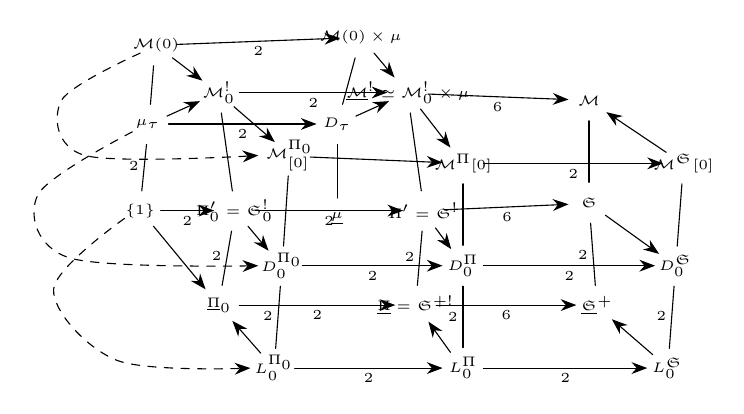
\begin{tikzpicture}[x=1mm,y=1mm,line cap=round,line join=round,font=\scriptsize]
\node[inner sep=1pt] at (27,-12.6) {\tiny $\mathcal M(0)$};
\node[inner sep=1pt] at (53,-11.6) {\tiny $\mathcal M(0)\times\mu$};
\node[inner sep=1pt] at (35,-18.6) {\tiny $\mathcal M^!_0$};
\node[inner sep=1pt] at (59,-18.6) {\tiny $\underline{\mathcal M}^!\simeq\mathcal M^!_0\times\mu$};
\node[inner sep=1pt] at (82,-19.6) {\tiny $\mathcal M$};
\node[inner sep=1pt] at (44,-26.6) {\tiny $\mathcal M^{\Pi_0}_{[0]}$};
\node[inner sep=1pt] at (66,-27.6) {\tiny $\mathcal M^{\Pi}[0]$};
\node[inner sep=1pt] at (94,-27.6) {\tiny $\mathcal M^{\mathfrak S}[0]$};
\node[inner sep=1pt] at (26,-22.6) {\tiny $\mu_\tau$};
\node[inner sep=1pt] at (50,-22.6) {\tiny $D_\tau$};
\node[inner sep=1pt] at (25,-33.6) {\tiny $\{1\}$};
\node[inner sep=1pt] at (37,-33.6) {\tiny $\Pi'_0=\mathfrak S^!_0$};
\node[inner sep=1pt] at (50,-34.6) {\tiny $\underline\mu$};
\node[inner sep=1pt] at (61,-33.6) {\tiny $\Pi'=\mathfrak S^!$};
\node[inner sep=1pt] at (82,-32.6) {\tiny $\mathfrak S$};
\node[inner sep=1pt] at (43,-40.6) {\tiny $D^{\Pi_0}_0$};
\node[inner sep=1pt] at (66,-40.6) {\tiny $D^{\Pi}_0$};
\node[inner sep=1pt] at (93,-40.6) {\tiny $D^{\mathfrak S}_0$};
\node[inner sep=1pt] at (35,-45.6) {\tiny $\underline\Pi_0$};
\node[inner sep=1pt] at (60,-45.6) {\tiny $\underline\Pi=\mathfrak S^{+!}$};
\node[inner sep=1pt] at (83,-45.6) {\tiny $\underline{\mathfrak S}^+$};
\node[inner sep=1pt] at (42,-53.6) {\tiny $L^{\Pi_0}_0$};
\node[inner sep=1pt] at (66,-53.6) {\tiny $L^{\Pi}_0$};
\node[inner sep=1pt] at (92,-53.6) {\tiny $L^{\mathfrak S}_0$};
\draw[-{Stealth[length=2mm]}] (29.6,-12.5) -- (50.4,-11.7);
\node[inner sep=1pt] at (40,-13.4) {\tiny $2$};
\draw[-{Stealth[length=2mm]}] (37.6,-18.6) -- (56.4,-18.6);
\node[inner sep=1pt] at (47,-19.9) {\tiny $2$};
\draw[-{Stealth[length=2mm]}] (61.6,-18.8) -- (79.4,-19.5);
\node[inner sep=1pt] at (70.4,-20.4) {\tiny $6$};
\draw[-{Stealth[length=2mm]}] (46.6,-26.8) -- (63.4,-27.5);
\draw[-{Stealth[length=2mm]}] (68.6,-27.6) -- (91.4,-27.6);
\node[inner sep=1pt] at (80,-28.9) {\tiny $2$};
\draw (26.7,-15.2) -- (26.3,-20.1);
\draw (52.3,-14.2) -- (50.7,-20.1);
\draw (35.3,-21.2) -- (36.7,-31.1);
\draw (59.3,-21.2) -- (60.7,-31.1);
\draw (82,-22.2) -- (82,-30);
\draw (43.8,-29.2) -- (43.2,-38.1);
\draw (66,-30.2) -- (66,-38);
\draw (93.8,-30.2) -- (93.2,-38.1);
\draw[-{Stealth[length=2mm]}] (29.1,-14.2) -- (32.9,-17.1);
\draw[-{Stealth[length=2mm]}] (54.7,-13.6) -- (57.3,-16.7);
\draw[-{Stealth[length=2mm]}] (36.9,-20.4) -- (42.1,-24.9);
\draw[-{Stealth[length=2mm]}] (60.6,-20.7) -- (64.4,-25.6);
\draw[-{Stealth[length=2mm]}] (91.8,-26.2) -- (84.2,-21.1);
\draw[-{Stealth[length=2mm]}] (28.6,-22.6) -- (47.4,-22.6);
\node[inner sep=1pt] at (38,-23.9) {\tiny $2$};
\draw[-{Stealth[length=2mm]}] (27.6,-33.6) -- (34.4,-33.6);
\node[inner sep=1pt] at (31,-34.9) {\tiny $2$};
\draw[-{Stealth[length=2mm]}] (39.6,-33.6) -- (58.4,-33.6);
\node[inner sep=1pt] at (49,-34.9) {\tiny $2$};
\draw[-{Stealth[length=2mm]}] (63.6,-33.5) -- (79.4,-32.8);
\node[inner sep=1pt] at (71.6,-34.4) {\tiny $6$};
\draw[-{Stealth[length=2mm]}] (45.6,-40.6) -- (63.4,-40.6);
\node[inner sep=1pt] at (54.5,-41.9) {\tiny $2$};
\draw[-{Stealth[length=2mm]}] (68.6,-40.6) -- (90.4,-40.6);
\node[inner sep=1pt] at (79.5,-41.9) {\tiny $2$};
\draw (25.8,-25.2) -- (25.2,-31.1);
\node[inner sep=1pt] at (24.2,-28) {\tiny $2$};
\draw (50,-25.2) -- (50,-32);
\draw[-{Stealth[length=2mm]}] (38.7,-35.6) -- (41.3,-38.7);
\draw[-{Stealth[length=2mm]}] (62.5,-35.8) -- (64.5,-38.5);
\draw[-{Stealth[length=2mm]}] (84.1,-34.2) -- (90.9,-39.1);
\draw[-{Stealth[length=2mm]}] (28.4,-21.6) -- (32.6,-19.7);
\draw[-{Stealth[length=2mm]}] (52.4,-21.6) -- (56.6,-19.7);
\draw[-{Stealth[length=2mm]}] (37.6,-45.6) -- (57.4,-45.6);
\node[inner sep=1pt] at (47.5,-46.9) {\tiny $2$};
\draw[-{Stealth[length=2mm]}] (62.6,-45.6) -- (80.4,-45.6);
\node[inner sep=1pt] at (71.5,-46.9) {\tiny $6$};
\draw[-{Stealth[length=2mm]}] (44.6,-53.6) -- (63.4,-53.6);
\node[inner sep=1pt] at (54,-54.9) {\tiny $2$};
\draw[-{Stealth[length=2mm]}] (68.6,-53.6) -- (89.4,-53.6);
\node[inner sep=1pt] at (79,-54.9) {\tiny $2$};
\draw (42.8,-43.2) -- (42.2,-51.1);
\node[inner sep=1pt] at (41.2,-47) {\tiny $2$};
\draw (66,-43.2) -- (66,-51);
\node[inner sep=1pt] at (64.7,-47.1) {\tiny $2$};
\draw (92.8,-43.2) -- (92.2,-51.1);
\node[inner sep=1pt] at (91.2,-47) {\tiny $2$};
\draw (36.6,-36.2) -- (35.4,-43.1);
\node[inner sep=1pt] at (34.7,-39.4) {\tiny $2$};
\draw (60.8,-36.2) -- (60.2,-43.1);
\node[inner sep=1pt] at (59.2,-39.5) {\tiny $2$};
\draw (82.2,-35.2) -- (82.8,-43.1);
\node[inner sep=1pt] at (81.2,-39.2) {\tiny $2$};
\draw[-{Stealth[length=2mm]}] (40.3,-51.7) -- (36.7,-47.6);
\draw[-{Stealth[length=2mm]}] (64.4,-51.6) -- (61.6,-47.7);
\draw[-{Stealth[length=2mm]}] (90.1,-51.9) -- (84.9,-47.4);
\draw[-{Stealth[length=2mm]}] (26.7,-35.6) -- (33.3,-43.6);
\draw[dashed,-{Stealth[length=2mm]}] plot[smooth, tension=0.55] coordinates {(25,-13.6) (15,-19.6) (18,-26.6) (40,-26.6)};
\draw[dashed,-{Stealth[length=2mm]}] plot[smooth, tension=0.55] coordinates {(24,-23.6) (12,-31.6) (16,-39.6) (40,-40.6)};
\draw[dashed,-{Stealth[length=2mm]}] plot[smooth, tension=0.55] coordinates {(23,-34.6) (14,-43.6) (22,-52.6) (39,-53.6)};
\end{tikzpicture}
\end{document}
